\documentclass[12pt,a4paper]{report}
\usepackage[french]{babel}
\usepackage[T1]{fontenc}
\usepackage[utf8]{inputenc}
\usepackage[skip=6pt]{parskip}
\usepackage{geometry}
\usepackage{footnote}
\usepackage{graphicx}
\usepackage{hyperref}
\usepackage{bookmark}
\usepackage{setspace}
\usepackage{fancyhdr}
\usepackage{titlesec} % Pour définir les tailles des titres
\usepackage{mathptmx} % Utiliser Times New Roman
\usepackage{ragged2e} % Pour justifier le texte
\usepackage{setspace}  % Pour gérer l'interligne
\geometry{top=3cm, bottom=3cm, left=3cm, right=3cm}
\hypersetup{hidelinks}
\pagestyle{fancy}
\fancyhf{}
\cfoot{\thepage} % Centrer la numérotation de page en bas de page
\hypersetup{
    colorlinks=true,
    linkcolor=blue,
    filecolor=magenta,      
    urlcolor=cyan,
    pdftitle={Mémoire de Fin d'Études},
    pdfpagemode=FullScreen,
}

% Définir les tailles des titres
\titleformat{\chapter}[hang]{\normalfont\fontsize{14}{16}\selectfont}{\thechapter.}{1em}{\fontsize{14}{16}\selectfont} % 14 pt pour les gros titres
\titleformat{\section}[hang]{\normalfont\fontsize{13}{15}\selectfont}{\thesection.}{1em}{\fontsize{13}{15}\selectfont} % 13 pt pour les sous-titres
\titleformat{\subsection}[hang]{\normalfont\fontsize{12}{14}\selectfont}{\thesubsection.}{1em}{\fontsize{12}{14}\selectfont} % 12 pt pour les sous-sous-titres

% Définir la taille du texte
\renewcommand{\normalsize}{\fontsize{11}{13}\selectfont} % 11 pt pour le texte

% Définir la taille des notes de bas de page
\renewcommand{\footnotesize}{\fontsize{10}{12}\selectfont} % 10 pt pour les notes

% Définir la taille de la pagination
\fancyfoot[C]{\fontsize{9}{11}\selectfont \thepage} % 9 pt pour la pagination

\begin{document}
\justifying % Justifier le texte
\onehalfspacing % Définir l'interligne à 1,5 pt
\addtolength{\parskip}{6pt} % Définit l'espacement entre les paragraphes
\setlength{\parindent}{15pt} % Définit l'indentation

% Page de garde
\begin{titlepage}
    \begin{center}
        \vspace*{\fill}

                % Logo de l'école
                
\includegraphics[width=0.3\textwidth]{images/logo.png}\\[1cm]
                
                {\Large \textbf{École Hexagone}}\\[0.5cm]
                {\small Mastère Architecture des Systèmes d'Information}\\[0.5cm]

                \rule{\linewidth}{0.5mm}\\[1cm]
                
                {\LARGE \textbf{Assistant intelligent pour la mémorisation}} \\[0.5cm]
                {\Large Comment l'intelligence artificielle peut-elle améliorer l'assistance à la mémorisation et l'accessibilité cognitive ?}\\[0.5cm]

                \rule{\linewidth}{0.5mm}\\[1cm]
                
                \textbf{Mémoire de fin d'études réalisé par}\\
                {\Large Valentin POIGT}\\[1cm]
                
                \textbf{Encadré par}\\
                {\Large Docteur Cyril-Alexandre PACHON}\\[0.5cm]

                \vspace*{\fill}
                
                {\Large Année universitaire 2024 – 2025}
        \vspace*{\fill}
    \end{center}
\end{titlepage}

% Résumé
\chapter*{Résumé}
\addcontentsline{toc}{chapter}{Résumé}

% Sommaire
\chapter*{Sommaire}
\addcontentsline{toc}{chapter}{Sommaire}
\tableofcontents

% Liste des figures et tableaux
\listoffigures
\listoftables
\newpage

% Glossaire (optionnel)
\chapter*{Glossaire}
\addcontentsline{toc}{chapter}{Glossaire}

\textbf{Intelligence artificielle (IA)} : Domaine de l'informatique visant à développer des systèmes capables de simuler l'intelligence humaine.

\textbf{Mémoire à court terme (MCT)} : Capacité de conserver temporairement des informations pendant une courte durée.

\textbf{Mémoire à long terme (MLT)} : Système de stockage des informations sur une période prolongée.

\textbf{Trouble du déficit de l'attention avec ou sans hyperactivité (TDAH)} : Trouble neurodéveloppemental caractérisé par des difficultés d'attention, d'impulsivité et, parfois, d'hyperactivité.

\textbf{Dyslexie} : Trouble spécifique de l'apprentissage de la lecture, se manifestant par des difficultés à identifier les mots et à lire de manière fluide.

\textbf{Surcharge cognitive} : Situation dans laquelle la quantité d'informations à traiter dépasse la capacité de traitement du cerveau.

\textbf{Maladie d'Alzheimer} : Maladie neurodégénérative caractérisée par une dégénérescence neuronale et une détérioration cognitive progressive.

\textbf{Maladie de Parkinson} : Maladie neurodégénérative provoquant des troubles moteurs et cognitifs dus à la perte de neurones dopaminergiques.

\textbf{Répétition espacée} : Méthode d'apprentissage consistant à réviser régulièrement les informations pour favoriser leur mémorisation à long terme.

\textbf{Traitement du langage naturel (NLP)} : Domaine de l'intelligence artificielle visant à permettre aux machines de comprendre, d'interpréter et de générer un langage humain.

% Remerciements
\chapter*{Remerciements}
\addcontentsline{toc}{chapter}{Remerciements}

% Introduction
\chapter*{Introduction}
\addcontentsline{toc}{chapter}{Introduction}

La mémoire constitue une fonction cognitive essentielle pour l'être humain. Elle permet d'acquérir, de stocker et de restituer des informations nécessaires à la vie quotidienne. Sans cette capacité, l'apprentissage deviendrait impossible et l'adaptation à un environnement en constante évolution serait fortement limitée. Pourtant, la mémoire n'est pas infaillible. De nombreux facteurs influencent son efficacité. Le stress, la surcharge cognitive, les troubles neurologiques ou encore l'âge altèrent la capacité à retenir des informations de manière durable.

L'augmentation de la quantité d'informations disponibles dans le monde numérique moderne impose de nouvelles contraintes. Assimiler et retenir des données devient une tâche de plus en plus complexe. Face à cette problématique, l'intelligence artificielle (IA) représente une opportunité pour compenser certaines limites cognitives et optimiser les processus de mémorisation. Grâce aux avancées technologiques en apprentissage automatique, en traitement du langage naturel et en reconnaissance vocale, il est désormais possible de concevoir des outils capables de structurer, d'adapter et de restituer des connaissances en fonction des besoins spécifiques de chaque individu.

Les technologies d'IA sont déjà présentes dans plusieurs domaines. Les assistants conversationnels, les plateformes d'apprentissage adaptatif et les systèmes de rappel intelligent sont utilisés pour améliorer l'accès aux informations. Les applications dédiées à l'éducation exploitent ces innovations pour adapter les contenus pédagogiques en fonction des profils des apprenants. L'IA trouve également une application dans la santé cognitive. Des outils spécialisés assistent les personnes atteintes de troubles de la mémoire en leur proposant des rappels automatisés et des exercices de stimulation cognitive.

Cependant, malgré ces avancées, des questions subsistent. L'IA est-elle réellement capable d'améliorer la mémorisation et de faciliter l'accès aux connaissances ? Ces solutions sont-elles accessibles à tous et adaptées aux différents profils d'utilisateurs ? Quels sont les défis techniques et éthiques liés à leur utilisation ?

\newpage
Ce mémoire vise à répondre à ces interrogations en structurant l'analyse autour de trois axes. Tout d'abord, il est essentiel de comprendre les mécanismes de la mémoire humaine, ses limites et les défis rencontrés dans l'acquisition et la rétention d'informations. Ensuite, l'étude des technologies d'IA appliquées à la mémoire permet d'identifier les outils existants et d'évaluer leur efficacité. Enfin, l'analyse des applications concrètes et des enjeux liés à ces solutions apporte un éclairage sur les défis éthiques, techniques et ergonomiques, ainsi que sur les perspectives d'évolution dans ce domaine.

Ainsi, ce mémoire s'attache à explorer le potentiel de l'IA pour améliorer l'assistance à la mémorisation et l'accessibilité cognitive, tout en mettant en avant les opportunités et les limites de ces technologies. L'objectif est d'identifier des pistes d'amélioration permettant d'optimiser ces outils et de garantir une utilisation éthique et efficace au service des utilisateurs.

% 1
\chapter{La mémoire humaine et ses limites}

%1.1
\section{Les mécanismes de la mémoire}

%1.1.1
\subsection{Définition et fonctionnement de la mémoire}

La mémoire est une fonction cognitive essentielle qui nous permet d'enregistrer, de conserver et de restituer des informations issues de nos expériences et de notre environnement. Elle est au cœur de notre identité, de notre capacité d'apprentissage et de notre adaptation au monde qui nous entoure.

La mémoire humaine est un processus complexe qui implique l'encodage, le stockage et la récupération d'informations. Elle ne se limite pas à un simple enregistrement passif des données, mais est un processus actif qui transforme et organise les informations pour les rendre utilisables. Cette capacité nous permet de nous souvenir d'événements passés, d'acquérir de nouvelles connaissances et de développer des compétences.
\cite{mnpaf}

% 1.1.2
\subsection{Les systèmes de mémoire}

Les chercheurs ont identifié plusieurs types de mémoire qui interagissent pour assurer le traitement de l'information. Ces systèmes sont généralement classés en fonction de la durée de rétention et de la nature des informations traitées.
\cite{frcneurodon}

\textbf{La mémoire sensorielle} est la capacité à retenir des informations sensorielles pendant une très courte durée, généralement inférieure à une seconde. Elle agit comme un tampon qui enregistre fidèlement les stimuli sensoriels avant qu'ils ne soient traités par la mémoire à court terme. Par exemple, la mémoire iconique retient une image visuelle pendant une fraction de seconde après sa disparition, tandis que la mémoire échoïque conserve une trace auditive pendant quelques instants.

\textbf{La mémoire à court terme (MCT)}, également appelée mémoire de travail, est responsable du stockage temporaire et de la manipulation des informations nécessaires aux activités cognitives quotidiennes, telles que la compréhension, le raisonnement et l'apprentissage. Elle a une capacité limitée et une durée de rétention brève.

\newpage
\textbf{Caractéristiques de la MCT :}
\begin{itemize}
    \item \textbf{Capacité limitée :} La mémoire à court terme peut retenir environ 7 éléments différents simultanément.
    \item \textbf{Durée brève :} L'information y est conservée entre 0,5 seconde et 10 minutes en l'absence de répétition.
    \item \textbf{Nature fragile :} Toute distraction ou surcharge cognitive peut entraîner l'oubli de l'information stockée.
\end{itemize}

\textbf{Le modèle de Baddeley et Hitch (1974)} a proposé une vision plus détaillée de la mémoire à court terme, en introduisant le concept de mémoire de travail. Ce modèle considère la mémoire de travail comme un système dynamique qui permet la manipulation des informations pour des tâches complexes comme la résolution de problèmes.

\begin{figure}[h]
    \centering
    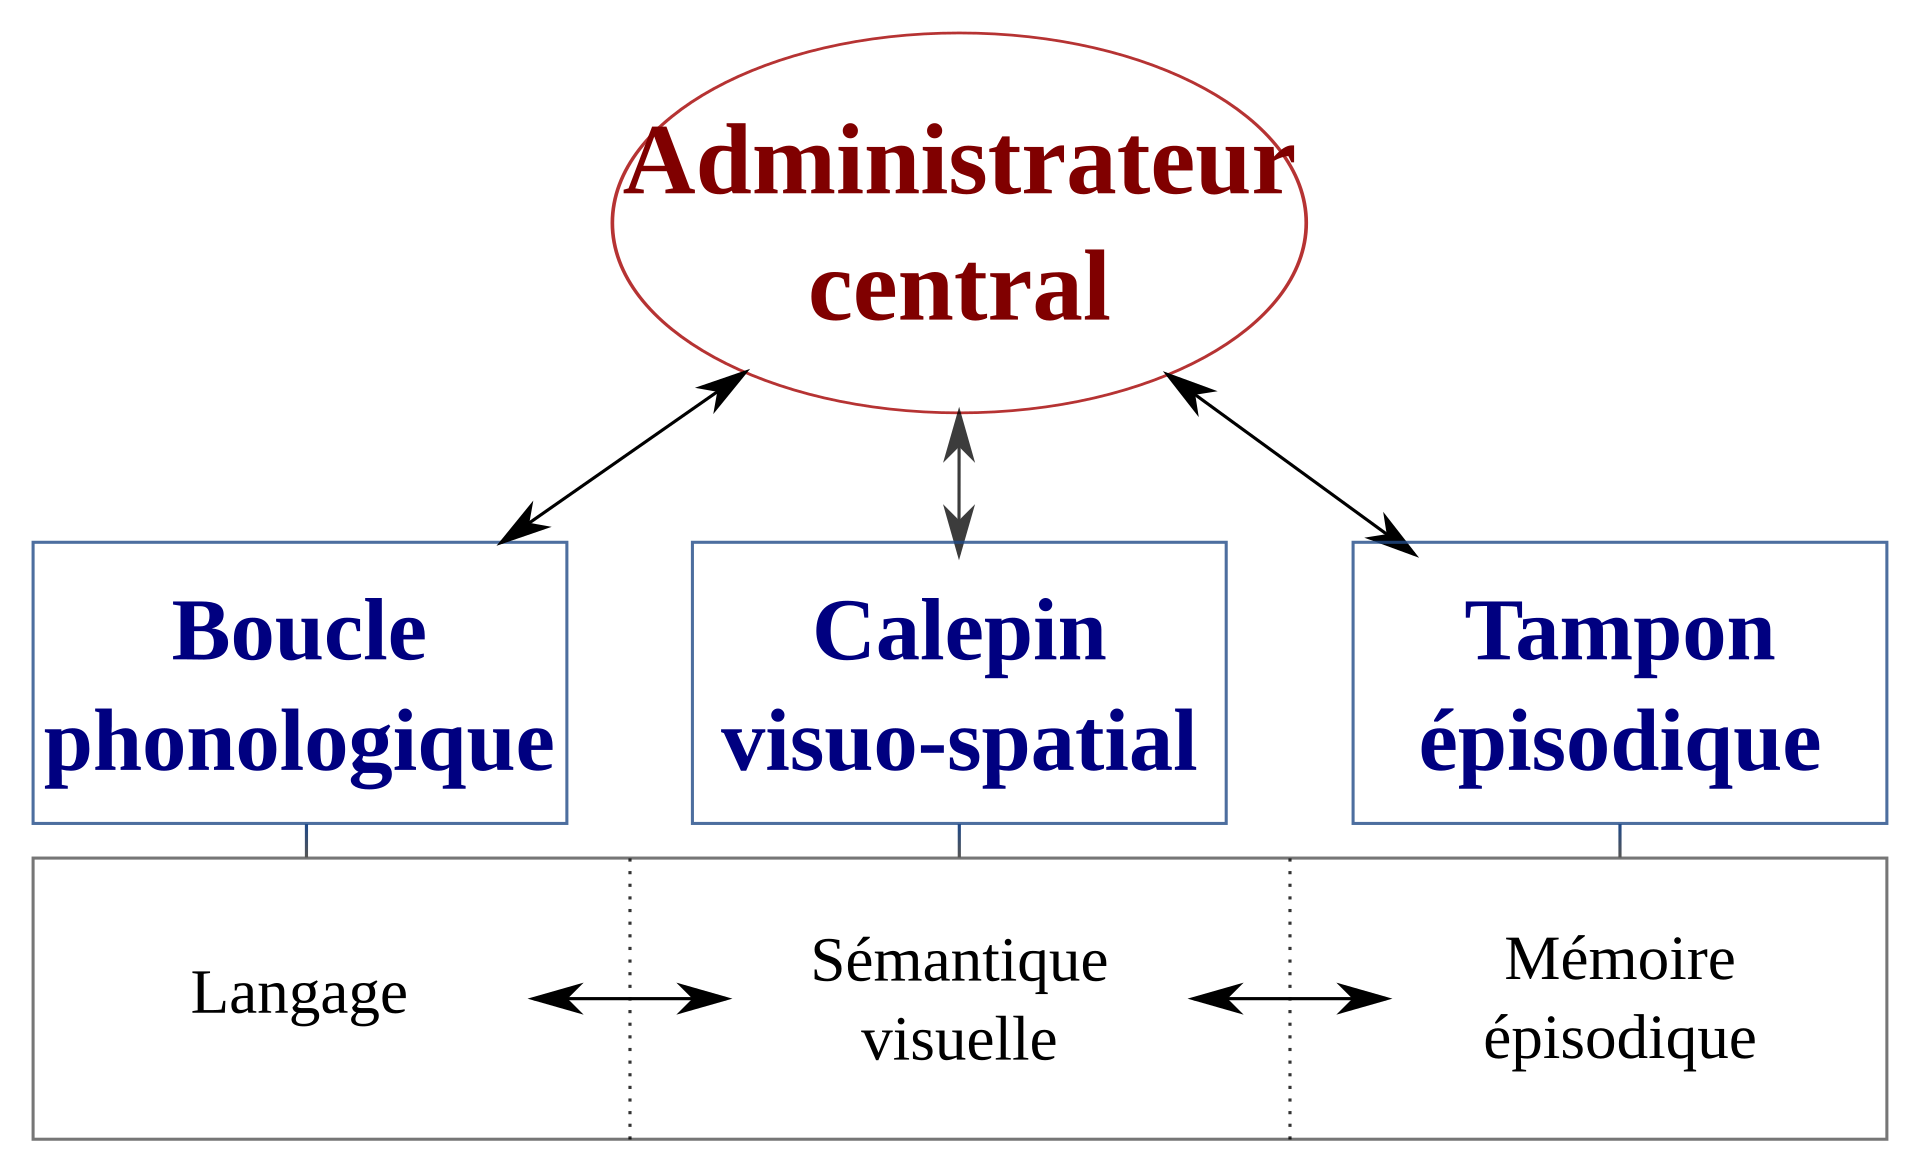
\includegraphics[width=0.7\textwidth]{images/modele_baddeley_hitch.png}
    \caption{Schéma du modèle de la mémoire de travail selon Baddeley et Hitch}
    \label{fig:baddeley}
\end{figure}

\newpage
Contrairement à la mémoire à court terme (MCT), \textbf{la mémoire à long terme (MLT)} stocke les informations de manière potentiellement illimitée et pour une durée prolongée. Elle permet d'accumuler des connaissances, des expériences et des souvenirs sur plusieurs années.

\textbf{Types de mémoire à long terme :}
\begin{itemize}
    \item \textbf{Mémoire déclarative (explicite) :} Elle concerne les souvenirs accessibles à la conscience et pouvant être exprimés verbalement.
    \begin{itemize}
        \item \textbf{Mémoire épisodique :} Stocke des souvenirs personnels, tels que des événements vécus (par exemple, un anniversaire d'enfance).
        \item \textbf{Mémoire sémantique :} Contient des connaissances générales sur le monde (par exemple, savoir que la Tour Eiffel se trouve à Paris).
    \end{itemize}
    \item \textbf{Mémoire non déclarative (implicite) :} Elle fonctionne sans implication consciente et se manifeste par des habiletés motrices ou des automatismes.
    \begin{itemize}
        \item \textbf{Mémoire procédurale :} Responsable de l'apprentissage des gestes et des compétences (par exemple, faire du vélo).
        \item \textbf{Conditionnements et habitudes :} Permet de réagir de manière automatique à certains stimuli (par exemple, saliver à l'odeur d'un plat préféré).
    \end{itemize}
\end{itemize}

\begin{figure}[h]
    \centering
    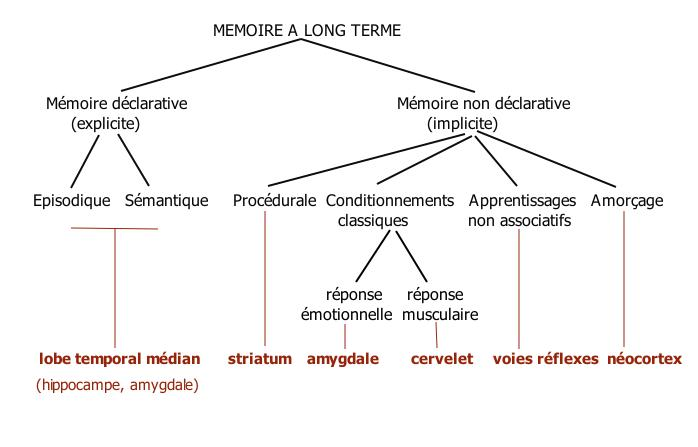
\includegraphics[width=0.7\textwidth]{images/types_memoire_long_terme.jpg}
    \caption{Représentation schématique des types de mémoire à long terme}
    \label{fig:mlt}
\end{figure}

\newpage
% 1.1.3
\subsection{Lien entre mémoire à court terme et mémoire à long terme}

La mémoire à court terme et la mémoire à long terme ne fonctionnent pas de manière indépendante, mais forment un système intégré. Le transfert d'informations entre ces deux systèmes est influencé par plusieurs facteurs, notamment :

\begin{itemize}
    \item \textbf{L'attention :} Une information qui capte fortement l'attention a plus de chances d'être stockée durablement.
    \item \textbf{La répétition :} La répétition espacée améliore la consolidation mnésique.
    \item \textbf{L'émotion :} Un événement émotionnellement marquant est plus susceptible d'être stocké dans la mémoire à long terme.
\end{itemize}

Des études ont montré que l'hippocampe, une structure cérébrale essentielle, joue un rôle clé dans le passage de la mémoire à court terme vers la mémoire à long terme.
\cite{humanite}


% 1.2
\section{Les troubles de la mémoire et leurs impacts}

% 1.2.1
\subsection{Vieillissement cognitif et maladies neurodégénératives}

La mémoire humaine est sujette à diverses altérations résultant de facteurs tels que le vieillissement, les maladies neurodégénératives, les troubles de l'attention et de l'apprentissage, ainsi que la surcharge cognitive. Ces perturbations ont des répercussions significatives sur la qualité de vie des individus concernés.

Le vieillissement naturel entraîne un déclin progressif des capacités cognitives, affectant notamment la mémoire, l'apprentissage et la rapidité de traitement de l'information. Ce processus est accentué par des pathologies neurodégénératives comme la maladie d'Alzheimer et la maladie de Parkinson.

La maladie d'Alzheimer est caractérisée par une accumulation anormale de protéines bêta-amyloïdes et tau dans le cerveau, conduisant à une dégénérescence neuronale et à une détérioration cognitive progressive.\cite{dr_calon} Elle représente plus de 70 \% des cas de démence chez les personnes âgées.\cite{ess_autonomie}

La maladie de Parkinson, quant à elle, est marquée par la perte de neurones dopaminergiques dans la substantia nigra, entraînant des troubles moteurs et cognitifs. Bien que principalement associée à des symptômes moteurs, cette pathologie peut également affecter la mémoire et d'autres fonctions cognitives.

\newpage

% 1.2.2
\subsection{Troubles de l'attention et de l'apprentissage}

Les troubles de l'attention, tels que le trouble du déficit de l'attention avec ou sans hyperactivité (TDAH), et les troubles spécifiques de l'apprentissage, comme la dyslexie, impactent significativement la capacité de mémorisation et d'acquisition des connaissances. \ref{fig:tdah}

Le TDAH se manifeste par des difficultés à maintenir l'attention, une impulsivité et, parfois, une hyperactivité. Ces symptômes entravent la capacité à se concentrer sur des tâches spécifiques, affectant ainsi l'apprentissage et la mémorisation. Il est fréquent que le TDAH coexiste avec des troubles de l'apprentissage, notamment la dyslexie. \cite{dyscoaching}

La dyslexie est un trouble spécifique de l'apprentissage de la lecture, caractérisé par des difficultés à identifier les mots, à lire de manière fluide et à orthographier correctement. Ces défis peuvent entraîner une faible estime de soi et une aversion pour les activités liées à la lecture, limitant ainsi l'exposition à de nouvelles informations et, par conséquent, la capacité de mémorisation. \cite{tdah}

% 1.2.3
\subsection{Surcharge cognitive et oubli informationnel}

La surcharge cognitive survient lorsque la quantité d'informations à traiter dépasse la capacité de traitement du cerveau, conduisant à une diminution de l'efficacité de la mémorisation. Dans notre société moderne, l'exposition constante à une multitude de stimuli et d'informations peut entraîner une surcharge cognitive, rendant difficile la sélection et la consolidation des informations pertinentes.

L'oubli informationnel est souvent une conséquence directe de cette surcharge. \cite{dyscoaching} Lorsque le cerveau est submergé par trop d'informations, il peut ne pas être en mesure de les encoder correctement en mémoire à long terme, ce qui conduit à un oubli rapide. Des stratégies telles que la gestion efficace du temps, la priorisation des tâches et l'utilisation d'outils d'organisation peuvent aider à atténuer les effets de la surcharge cognitive et à améliorer la rétention d'informations.

\newpage

%1.3
\section{Besoins et solutions existantes pour améliorer la mémorisation}

%1.3.1
\subsection{Méthodes traditionnelles et techniques mnémotechniques}

La capacité à mémoriser efficacement est essentielle dans de nombreux domaines, qu'il s'agisse de l'éducation, du milieu professionnel ou de la vie quotidienne. Face aux défis posés par la quantité croissante d'informations à assimiler, diverses méthodes ont été développées pour optimiser la mémorisation. Ces approches incluent des techniques traditionnelles, l'utilisation des technologies numériques actuelles et une réflexion sur les limites des méthodes classiques.

Parmi les techniques éprouvées pour améliorer la mémoire, les méthodes mnémotechniques et la répétition espacée occupent une place prépondérante.

Les méthodes mnémotechniques consistent à utiliser des associations mentales pour faciliter la mémorisation. Par exemple, l'acronyme "MERCREDI" peut aider à retenir les noms des planètes du système solaire dans l'ordre croissant de leur distance au Soleil : Mercure, Vénus, Terre, Mars, Jupiter, Saturne, Uranus, Neptune. Ces techniques exploitent la capacité du cerveau à se souvenir plus facilement d'images, de rimes ou d'histoires que d'informations brutes. \cite{hiphiphip}

La répétition espacée est une méthode basée sur la courbe de l'oubli d'Ebbinghaus, qui démontre que la mémorisation s'améliore avec le nombre de répétitions, et que l'oubli recule en conséquence. Cette technique consiste à réviser l'information à des intervalles de temps croissants, renforçant ainsi la mémorisation à long terme. Par exemple, après une première lecture, une révision peut être effectuée le lendemain, puis trois jours plus tard, une semaine après, et ainsi de suite. Cette approche permet de consolider l'information dans la mémoire à long terme en exploitant l'effet d'espacement. \cite{memoriclub} \cite{lectureincr}

%1.3.2
\subsection{Utilisation des technologies numériques actuelles}

Avec l'avènement du numérique, de nouvelles solutions ont émergé pour faciliter la mémorisation. Les applications de flashcards numériques, comme Anki ou Quizlet, permettent aux utilisateurs de créer des cartes mémoire interactives et d'appliquer la répétition espacée de manière automatisée. Ces outils offrent une flexibilité accrue et une personnalisation des contenus à mémoriser.

Les applications de révision active, telles que DIGIFLASHCARDS, proposent des fonctionnalités interactives pour la révision, combinant des techniques telles que la répétition espacée, les révisions croisées et le mind mapping. Ces outils numériques permettent une adaptation aux besoins spécifiques de chaque apprenant, favorisant une mémorisation plus efficace. \cite{stewdy}

De plus, certaines plateformes éducatives intègrent des algorithmes d'apprentissage adaptatif qui ajustent le contenu et le rythme des révisions en fonction des performances de l'utilisateur. Cette personnalisation de l'apprentissage permet de cibler les lacunes spécifiques et d'optimiser le processus de mémorisation.

%1.3.3
\subsection{Limites des approches classiques}

Malgré leur efficacité, les méthodes traditionnelles de mémorisation présentent certaines limites. Elles peuvent être perçues comme monotones et manquer d'engagement, ce qui peut réduire la motivation de l'apprenant. De plus, ces techniques nécessitent une discipline et une régularité que tous ne parviennent pas à maintenir.

L'intégration des technologies numériques dans les pratiques pédagogiques peut également poser des défis. Bien que les outils numériques puissent constituer des appuis efficaces pour l'apprentissage, ils ne peuvent provoquer l'apprentissage seuls. La formation et l'accompagnement des enseignants pour intégrer ces outils dans des scénarios pédagogiques avec des visées d'apprentissage précises restent un enjeu majeur. \cite{res-canope}

Par ailleurs, une utilisation excessive des outils numériques peut entraîner une surcharge cognitive, affectant ainsi la qualité de la mémorisation. Il est donc essentiel de trouver un équilibre entre les méthodes traditionnelles et les technologies modernes pour optimiser l'apprentissage.

La mémorisation efficace repose sur une combinaison de méthodes traditionnelles éprouvées et de technologies numériques innovantes. Les techniques mnémotechniques et la répétition espacée offrent des bases solides pour l'apprentissage, tandis que les outils numériques apportent flexibilité et personnalisation. Cependant, il est crucial de reconnaître les limites de chaque approche et de les intégrer de manière réfléchie pour répondre aux besoins individuels des apprenants. Une utilisation équilibrée et informée de ces différentes méthodes peut ainsi conduire à une amélioration significative des capacités de mémorisation.

\newpage

%2
\chapter{L'intelligence artificielle au service de la mémorisation}

%2.1
\section{Présentation des technologies d'IA utilisées pour l'assistance cognitive}

%2.1.1
\subsection{Traitement du langage naturel (NLP)}

L'intelligence artificielle (IA) a révolutionné de nombreux domaines, notamment celui de l'assistance cognitive. Parmi les technologies d'IA les plus influentes dans ce contexte figurent le traitement du langage naturel (NLP), l'apprentissage automatique et adaptatif, ainsi que la reconnaissance vocale et la synthèse de la parole. Ces avancées technologiques ont permis le développement d'outils et de systèmes capables d'interagir de manière plus intuitive et efficace avec les utilisateurs, améliorant ainsi leur expérience et leur productivité.

Le traitement du langage naturel est une branche de l'IA qui se concentre sur l'interaction entre les ordinateurs et les humains à travers le langage naturel. Il englobe diverses tâches, telles que la compréhension, la génération et la traduction automatiques du langage humain. Dans le cadre de l'assistance cognitive, le NLP permet aux systèmes de comprendre et de répondre aux requêtes des utilisateurs de manière contextuelle et pertinente. Par exemple, des assistants virtuels comme Siri ou Alexa utilisent le NLP pour interpréter les commandes vocales et fournir des réponses appropriées. De plus, des applications comme Rogervoice exploitent le NLP pour transcrire en temps réel les appels téléphoniques, rendant ainsi la communication plus accessible aux personnes sourdes ou malentendantes.

%2.1.2
\subsection{Apprentissage automatique et adaptatif}

L'apprentissage automatique, ou machine learning, est une composante clé de l'IA qui permet aux systèmes de s'améliorer automatiquement à partir de l'expérience sans être explicitement programmés. L'apprentissage adaptatif, quant à lui, est une approche où les modèles s'ajustent en temps réel en fonction des nouvelles données reçues, permettant une personnalisation accrue des services. Par exemple, des systèmes de recommandation personnalisés utilisent l'apprentissage adaptatif pour suggérer des contenus ou des produits en fonction des préférences et du comportement de l'utilisateur. Des institutions comme l'Institut de recherche Idiap en Suisse sont à la pointe de la recherche dans ces domaines, développant des algorithmes avancés pour améliorer l'efficacité et la précision des systèmes d'assistance cognitive.

%2.1.3
\subsection{Reconnaissance vocale et synthèse de la parole}

La reconnaissance vocale et la synthèse de la parole sont deux technologies complémentaires qui jouent un rôle crucial dans l'assistance cognitive. La reconnaissance vocale permet aux systèmes de convertir la parole humaine en texte, facilitant ainsi l'interaction homme-machine. Par exemple, des chercheurs comme Lawrence Rabiner ont contribué de manière significative au développement d'algorithmes de reconnaissance vocale, rendant possible des applications telles que la composition automatique d'appels téléphoniques. La synthèse de la parole, en revanche, consiste à convertir du texte en parole, permettant aux systèmes de communiquer verbalement avec les utilisateurs. Des laboratoires comme Grenoble Images Parole Signal Automatique (GIPSA-lab) en France ont mené des recherches approfondies dans ce domaine, développant des systèmes capables de reproduire la parole humaine de manière naturelle et expressive.

En combinant ces technologies, l'IA offre des solutions d'assistance cognitive de plus en plus sophistiquées, capables de comprendre, d'apprendre et de communiquer avec les utilisateurs de manière efficace et naturelle.


%2.2
\section{Les assistants intelligents pour la mémoire}

%2.2.1
\subsection{Présentation des outils et applications existantes}

L'évolution rapide de l'intelligence artificielle (IA) a conduit au développement d'assistants intelligents conçus pour améliorer nos capacités de mémorisation et de gestion des tâches quotidiennes. Ces outils, qu'ils soient intégrés dans des appareils ou disponibles sous forme d'applications, jouent un rôle crucial dans l'assistance cognitive. Parmi eux, les assistants vocaux, les systèmes de rappel intelligents et les applications de mémorisation se distinguent par leurs fonctionnalités et leur adaptabilité aux besoins des utilisateurs.

Les assistants vocaux sont des logiciels capables d'interagir avec les utilisateurs via des commandes vocales, facilitant ainsi l'accès à diverses informations et services.

\begin{itemize}
    \item Siri : Intégré aux appareils Apple, Siri permet d'effectuer des tâches telles que la définition de rappels, la recherche d'informations ou l'envoi de messages, simplement par la voix.

    \item Alexa : Développé par Amazon, Alexa est présent dans les appareils Echo et offre des fonctionnalités allant de la lecture de musique à la gestion de la domotique, en passant par la fourniture de mises à jour météorologiques.

    \item Google Assistant : Disponible sur les appareils Android et les enceintes connectées Google Home, Google Assistant aide les utilisateurs à planifier leurs journées, répondre à des questions et contrôler des appareils intelligents.
\end{itemize}

Ces assistants vocaux utilisent des technologies avancées de traitement du langage naturel pour comprendre et répondre aux requêtes des utilisateurs, améliorant ainsi leur expérience et leur efficacité.

Les systèmes de rappel intelligents sont conçus pour aider les utilisateurs à organiser leurs tâches et à se souvenir des événements importants.

\begin{itemize}
    \item Google Keep : Cette application permet de créer des notes, des listes et des rappels, avec la possibilité d'ajouter des images et des enregistrements vocaux. Elle offre une synchronisation en temps réel sur tous les appareils connectés à un compte Google.
    
    \item Todoist avec IA : Todoist est une application de gestion de tâches qui intègre l'intelligence artificielle pour proposer des priorités automatisées, des rappels intelligents et des analyses de productivité, aidant ainsi les utilisateurs à gérer efficacement leur charge de travail.
    
\end{itemize}

Ces outils s'adaptent aux habitudes et aux préférences des utilisateurs, offrant une expérience personnalisée qui facilite la gestion des tâches quotidiennes.

Pour ceux qui cherchent à améliorer leur capacité de mémorisation, plusieurs applications dédiées offrent des approches innovantes.

\begin{itemize}
    \item Anki : Basée sur le principe de la répétition espacée, Anki permet aux utilisateurs de créer des cartes mémoire personnalisées pour faciliter l'apprentissage et la rétention d'informations.
    \item Memrise : Cette application combine des techniques de mémorisation avec des contenus créés par la communauté pour aider les utilisateurs à apprendre de nouvelles langues et d'autres sujets de manière ludique et interactive.
    \item Duolingo : Principalement axée sur l'apprentissage des langues, Duolingo utilise des exercices interactifs et des rappels réguliers pour aider les utilisateurs à développer et maintenir leurs compétences linguistiques.
\end{itemize}

Ces applications exploitent des techniques pédagogiques éprouvées pour améliorer la mémorisation, rendant l'apprentissage plus accessible et efficace.

%2.2.2
\subsection{Fonctionnement et personnalisation des réponses en fonction des utilisateurs}

La personnalisation est au cœur de l'efficacité des assistants intelligents. En analysant les interactions passées, les préférences et les habitudes des utilisateurs, ces systèmes adaptent leurs réponses et leurs suggestions pour offrir une expérience sur mesure. Par exemple, un assistant vocal peut proposer des rappels basés sur l'historique des activités de l'utilisateur, tandis qu'une application de mémorisation peut ajuster la difficulté des exercices en fonction des performances précédentes. Cette adaptabilité améliore non seulement l'efficacité de ces outils, mais également l'engagement et la satisfaction des utilisateurs.

En conclusion, les assistants intelligents jouent un rôle essentiel dans l'amélioration de la mémoire et de la gestion des tâches quotidiennes. Qu'il s'agisse d'assistants vocaux, de systèmes de rappel intelligents ou d'applications de mémorisation, ces outils offrent des solutions personnalisées et efficaces pour répondre aux besoins variés des utilisateurs.

%2.3
\section{Avantages et limites de l'IA dans l'amélioration de la mémoire}

%2.3.1
\subsection{Amélioration de la rétention et de l'accessibilité de l'information}

L'intelligence artificielle (IA) a transformé notre manière d'interagir avec l'information, offrant des outils puissants pour améliorer la rétention et l'accessibilité des données. Cependant, cette avancée technologique s'accompagne de défis et de préoccupations qu'il est essentiel d'examiner.

L'IA excelle dans le traitement rapide et efficace de vastes quantités de données, surpassant les capacités humaines dans l'identification de schémas complexes et de relations subtiles entre les informations. Cette aptitude permet de structurer et de présenter les données de manière à faciliter leur compréhension et leur mémorisation. Par exemple, des systèmes d'apprentissage adaptatif exploitent l'IA pour personnaliser le contenu éducatif en fonction des besoins spécifiques de chaque apprenant, optimisant ainsi la rétention des connaissances.

De plus, l'IA offre une accessibilité accrue à l'information. Les assistants virtuels, tels que Siri ou Alexa, permettent aux utilisateurs d'accéder instantanément à des données ou des rappels, simplifiant la gestion des tâches quotidiennes et renforçant la mémoire externe. Cette disponibilité constante de l'information réduit la charge cognitive et libère des ressources mentales pour des activités plus complexes.

%2.3.2
\subsection{Adaptabilité et personnalisation}

L'un des atouts majeurs de l'IA réside dans sa capacité à s'adapter aux préférences et aux comportements individuels. Grâce à l'apprentissage automatique, les systèmes d'IA peuvent analyser les interactions passées d'un utilisateur pour proposer des solutions sur mesure. Par exemple, des applications éducatives utilisent l'IA pour ajuster le niveau de difficulté des exercices en fonction des performances de l'apprenant, favorisant ainsi une progression optimale.

Cette personnalisation ne se limite pas à l'éducation. Dans le domaine de la santé, l'IA peut analyser des données médicales pour recommander des traitements adaptés à chaque patient, améliorant ainsi l'efficacité des soins. Cette capacité d'adaptation rend l'IA particulièrement précieuse pour répondre aux besoins diversifiés des utilisateurs.

%2.3.3
\subsection{Risques et limites : dépendance technologique, confidentialité, biais algorithmiques}

Malgré ses avantages, l'IA présente des risques et des limitations qu'il convient de considérer.

\begin{itemize}
    \item Dépendance technologique : L'utilisation accrue de l'IA peut entraîner une dépendance excessive aux technologies, réduisant la capacité des individus à effectuer des tâches sans assistance numérique. Cette dépendance peut affecter les compétences cognitives et limiter l'autonomie personnelle.

    \item Confidentialité : Les systèmes d'IA collectent et analysent d'énormes volumes de données personnelles pour fonctionner efficacement. Cette collecte massive pose des questions sur la protection de la vie privée et le risque potentiel d'utilisation abusive des informations sensibles. Il est essentiel de mettre en place des réglementations strictes pour garantir la confidentialité des données des utilisateurs.

    \item Biais algorithmiques : Les algorithmes d'IA peuvent reproduire ou amplifier des biais présents dans les données d'entraînement, conduisant à des décisions injustes ou discriminatoires. Par exemple, un système de recrutement basé sur l'IA pourrait favoriser certains profils au détriment d'autres en raison de biais implicites dans les données historiques. Il est crucial de développer des algorithmes transparents et équitables pour éviter de tels problèmes.
\end{itemize}

En conclusion, l'IA offre des opportunités significatives pour améliorer la mémoire et l'accès à l'information grâce à ses capacités d'adaptation et de personnalisation. Cependant, il est impératif de reconnaître et d'aborder les défis associés, tels que la dépendance technologique, les préoccupations en matière de confidentialité et les biais algorithmiques, afin d'assurer une utilisation éthique et bénéfique de l'IA dans notre société.

%3
\chapter{Applications concrètes et enjeux éthiques}

%3.1
\section{L'IA dans l'éducation et l'apprentissage adaptatif}

%3.1.1
\subsection{Plateformes intelligentes pour l'éducation}

L'intelligence artificielle (IA) a profondément transformé le paysage éducatif en introduisant des outils et des plateformes capables de personnaliser l'apprentissage en fonction des besoins individuels des apprenants. Cette personnalisation est rendue possible grâce à l'analyse en temps réel des performances et à l'adaptation dynamique des contenus pédagogiques.

Des plateformes éducatives telles que Khan Academy et Coursera ont intégré l'IA pour offrir des expériences d'apprentissage plus personnalisées et efficaces.

\begin{itemize}

    \item Khan Academy : Cette plateforme utilise l'IA pour adapter les exercices et les leçons en fonction du niveau et des progrès de chaque élève. Par exemple, un algorithme de personnalisation dynamique intervient dès le premier exercice pour ajuster les contenus au plus près des besoins de l'apprenant.

    \item Coursera : En proposant des cours en ligne issus de diverses institutions, Coursera intègre l'IA pour analyser les interactions des utilisateurs et recommander des parcours d'apprentissage adaptés à leurs objectifs et à leurs performances.

\end{itemize}

%3.1.2
\subsection{Personnalisation de l'apprentissage en fonction des performances de l'utilisateur}

L'IA permet une personnalisation accrue de l'apprentissage en analysant les réponses et les progrès des apprenants pour ajuster le contenu pédagogique en temps réel. Cette approche, connue sous le nom d'apprentissage adaptatif, offre une expérience sur mesure à chaque individu.

\begin{itemize}
    \item Adaptation en temps réel : Les systèmes d'IA évaluent continuellement les performances des étudiants et modifient les exercices ou les leçons en fonction de leurs besoins spécifiques. Par exemple, un élève maîtrisant rapidement un concept peut se voir proposer des défis plus complexes, tandis qu'un autre nécessitant plus de temps recevra des explications supplémentaires. 
    \item Contenu personnalisé : Les plateformes éducatives utilisent l'IA pour créer des contenus adaptés aux styles d'apprentissage et aux préférences de chaque utilisateur, améliorant ainsi l'engagement et la rétention des connaissances.
\end{itemize}

\subsection{Suivi et analyse des progrès}

L'IA facilite le suivi détaillé des progrès des apprenants, permettant aux éducateurs et aux étudiants de mieux comprendre les domaines nécessitant une attention particulière.

\begin{itemize}
    \item Évaluation automatisée : Les outils d'IA peuvent corriger automatiquement les exercices et fournir un retour immédiat aux étudiants, accélérant ainsi le processus d'apprentissage. 
    \item Analyse prédictive : En examinant les données recueillies, l'IA peut identifier les tendances et prédire les difficultés potentielles, permettant une intervention proactive pour soutenir l'apprenant. 
\end{itemize}

En conclusion, l'intégration de l'IA dans l'éducation favorise une approche plus personnalisée et adaptative de l'apprentissage, répondant aux besoins spécifiques de chaque étudiant et améliorant l'efficacité des processus éducatifs.

%3.2
\section{L'IA pour les personnes atteintes de troubles cognitifs}

\subsection{Applications pour les seniors et les malades d'Alzheimer}

L'intelligence artificielle (IA) offre des perspectives prometteuses pour assister les individus souffrant de troubles cognitifs, qu'il s'agisse des seniors atteints de maladies neurodégénératives comme la maladie d'Alzheimer, des personnes vivant avec des troubles du déficit de l'attention avec ou sans hyperactivité (TDAH) ou la dyslexie, ainsi que celles confrontées à des déficiences mnésiques.

La maladie d'Alzheimer, une forme courante de démence, affecte la mémoire, la pensée et le comportement. L'IA intervient à plusieurs niveaux pour améliorer la qualité de vie des patients :

\begin{itemize}
    \item Diagnostic précoce : Des algorithmes d'apprentissage automatique analysent des données médicales complexes pour détecter précocement les signes de la maladie, permettant ainsi une intervention plus rapide.

    \item Applications de soutien : Des outils numériques, intégrant l'IA, aident les patients à gérer leurs routines quotidiennes, fournissent des rappels pour la prise de médicaments et facilitent la communication avec les soignants.

    \item Assistants virtuels : Des avatars interactifs, comme "Allison" développée par l'Alzheimer's Foundation of America, répondent aux questions des patients et de leurs familles, offrant des informations sur la maladie, des conseils en matière de santé cérébrale et un soutien aux aidants. 

\end{itemize}

%3.2.2
\subsection{Aide aux personnes atteintes de TDAH ou de dyslexie}

Pour les individus vivant avec le TDAH ou la dyslexie, l'IA propose des solutions adaptées :

\begin{itemize}

    \item Applications éducatives personnalisées : Des logiciels éducatifs adaptatifs ajustent le contenu en fonction des besoins spécifiques de l'utilisateur, améliorant ainsi l'engagement et l'efficacité de l'apprentissage.

    \item Outils de concentration : Des applications basées sur l'IA aident à gérer le temps, à organiser les tâches et à minimiser les distractions, soutenant ainsi les personnes avec TDAH dans leur vie quotidienne.

    \item Technologies d'assistance à la lecture : Des logiciels de reconnaissance vocale et de synthèse de la parole facilitent la lecture et l'écriture pour les personnes dyslexiques, en convertissant le texte en parole et vice versa.
\end{itemize}

%3.2.3
\subsection{Interfaces cerveau-ordinateur pour compenser les déficiences mnésiques}

Les interfaces cerveau-ordinateur (ICO) établissent une communication directe entre le cerveau et un dispositif externe, offrant des solutions innovantes pour compenser les déficiences mnésiques :

\begin{itemize}
    \item Restauration des fonctions perdues : Les ICO permettent aux individus ayant des troubles moteurs ou cognitifs sévères de contrôler des ordinateurs ou des prothèses par la pensée, améliorant ainsi leur autonomie. 

    \item Neurofeedback thérapeutique : Ces interfaces sont utilisées dans des approches thérapeutiques pour la rééducation fonctionnelle, aidant à récupérer des fonctions motrices ou cognitives altérées. 

    \item Perspectives futures : Des entreprises comme Paradromics explorent l'utilisation des ICO pour traiter des maladies neurodégénératives, améliorer la mémoire et potentiellement compenser les déficiences mnésiques. 
\end{itemize}

En conclusion, l'IA joue un rôle croissant dans l'assistance aux personnes atteintes de troubles cognitifs, offrant des outils et des technologies qui améliorent leur qualité de vie, favorisent leur autonomie et soutiennent leurs capacités cognitives.

%3.3
\section{Enjeux éthiques et défis techniques}

%3.3.1
\subsection{Confidentialité des données et respect de la vie privée}

L'introduction de l'intelligence artificielle (IA) dans divers domaines soulève des questions éthiques et techniques majeures. Parmi celles-ci, la confidentialité des données, la fiabilité des algorithmes, ainsi que l'accessibilité et l'inclusion occupent une place centrale.

L'IA repose sur l'analyse de vastes ensembles de données, souvent personnelles, ce qui pose des défis en matière de confidentialité et de protection de la vie privée. Les systèmes d'IA peuvent être vulnérables à des attaques visant à extraire des informations sensibles, compromettant ainsi la confidentialité des individus. Par ailleurs, l'utilisation de l'IA pour la surveillance de masse, notamment via la reconnaissance faciale, suscite des inquiétudes quant au respect de la vie privée.

%3.3.2
\subsection{Fiabilité et contrôle des algorithmes}

L'IA repose sur l'analyse de vastes ensembles de données, souvent personnelles, ce qui pose des défis en matière de confidentialité et de protection de la vie privée. Les systèmes d'IA peuvent être vulnérables à des attaques visant à extraire des informations sensibles, compromettant ainsi la confidentialité des individus. Par ailleurs, l'utilisation de l'IA pour la surveillance de masse, notamment via la reconnaissance faciale, suscite des inquiétudes quant au respect de la vie privée.

%3.2.3
\subsection{Accessibilité et inclusion : l'IA peut-elle être universellement efficace ?}

L'IA doit être conçue de manière à être accessible et bénéfique pour tous, indépendamment de l'origine, du genre ou du statut social. Cependant, des biais dans les données d'entraînement peuvent conduire à des systèmes discriminatoires, exacerbant les inégalités existantes. Par ailleurs, l'adoption de l'IA nécessite une infrastructure technologique adéquate, ce qui peut être un obstacle dans certaines régions ou pour certaines populations. Il est donc essentiel de promouvoir une conception inclusive de l'IA et de veiller à ce que ses bénéfices soient répartis équitablement.

En conclusion, le développement et l'intégration de l'IA doivent être accompagnés d'une réflexion approfondie sur les enjeux éthiques et techniques afin d'assurer une utilisation responsable et bénéfique pour l'ensemble de la société.

% Conclusion
\chapter*{Conclusion}
\addcontentsline{toc}{chapter}{Conclusion}
exemple\footnote{Ceci est une note de bas de page.}

L'intelligence artificielle (IA) a considérablement transformé notre manière d'interagir avec l'information, notamment en améliorant la mémorisation et les capacités cognitives. Les assistants intelligents, tels que ChatGPT, offrent des réponses rapides et précises, réduisant ainsi la surcharge cognitive et facilitant la prise de décision. Ces outils permettent une gestion plus efficace des informations, contribuant à une meilleure clarté mentale.

Les perspectives d'évolution des technologies d'IA dans le domaine de la mémorisation sont prometteuses. L'intégration de l'IA affective, capable de comprendre et de répondre aux émotions humaines, pourrait rendre les interactions avec les machines plus naturelles et empathiques. Cette avancée permettrait aux assistants virtuels de s'adapter davantage aux besoins individuels, enrichissant ainsi l'expérience utilisateur.

Cependant, des limites subsistent. Une dépendance excessive aux outils d'IA pourrait entraîner une diminution de l'engagement cognitif interne, affectant ainsi les compétences cognitives au fil du temps. De plus, des préoccupations concernant la confidentialité des données et la protection de la vie privée émergent, nécessitant une attention particulière pour assurer une utilisation éthique de l'IA.

Pour améliorer ces technologies, il est essentiel de développer des algorithmes transparents et explicables, renforçant ainsi la confiance des utilisateurs. De plus, garantir un accès équitable à ces outils est crucial pour éviter d'accentuer les inégalités existantes. Une conception inclusive de l'IA permettra de s'assurer que ses bénéfices profitent à l'ensemble de la société. 

En réfléchissant à l'impact futur des assistants intelligents sur la cognition humaine, il est probable que ces outils continueront à évoluer, offrant des interactions plus fluides et intuitives. Cependant, il est essentiel de trouver un équilibre entre l'utilisation de l'IA pour améliorer nos capacités cognitives et le maintien de nos compétences intrinsèques, afin de préserver notre autonomie intellectuelle. 

En somme, l'IA offre des opportunités significatives pour l'amélioration de la mémorisation et des capacités cognitives. Néanmoins, une approche réfléchie et éthique est nécessaire pour maximiser ses avantages tout en minimisant les risques potentiels.


% Bibliographie
\begin{thebibliography}{9}

    \bibitem{mnpaf} 
        MNPaf. Comment fonctionne notre mémoire. \break
        \url{https://www.mnpaf.fr/preserver-memoire/comment-fonctionne-notre-mémoire}

    \bibitem{francealzheimer} 
        France Alzheimer. Mémoire à long terme et mémoire à court terme. \break
        \url{https://www.francealzheimer.org/memoire-long-terme-court-terme/}
        
    \bibitem{humanite} 
        Humanité. L'hippocampe, siège de la mémoire et GPS de notre cerveau. \break
        \url{https://www.humanite.fr/sciences/academie-des-sciences/lhippocampe-siege-de-la-memoire-et-gps-de-notre-cerveau}
        
    \bibitem{frcneurodon} 
        FRC Neurodon. La mémoire. \break
        \url{https://www.frcneurodon.org/comprendre-le-cerveau/a-la-decouverte-du-cerveau/la-memoire/}

    \bibitem{ess_autonomie} 
        Malakoff, Humanis. (06/02/2025). Quelles sont les principales démences qui touchent les personnes âgées ? \textit{Essentiel autonomie}. \break
        \url{https://www.essentiel-autonomie.com/sante-mon-proche/quelles-sont-principales-demences-qui-touchent-personnes-agees}

    \bibitem{dr_calon}
        Dr. Calon. Maladie d'Alzheimer : causes, symptômes et traitements. \break
        \url{https://fr.wikipedia.org/wiki/Frédéric_Calon}
    
    \bibitem{dyscoaching}
        Dys-coaching. Trouble de déficit de l'attention. \break
        \url{https://www.dys-coaching.com/coin-parents/aide-pour-les-parents/trouble-de-deficit-de-l-attention/}

    \bibitem{tdah}
        L'ami TDAH. Mémoire de travail et TDAH. \break
    \url{https://www.laminicoachtdah.fr/vivre-avec-le-tdah/memoire-de-travail-et-tdah}

    \bibitem{hiphiphip}
        Blog HipHipHip. Guide pour mémoriser efficacement ses cours et réussir ses examens. \break
    \url{https://blog.hiphiphip.app/guides/guide-memoriser-efficacement-ses-cours-et-reussir-examens}

    \bibitem{memoriclub}
        Memori Club. Les répétitions espacées : meilleure technique de mémorisation. \break
    \url{https://memoriclub.com/memoire-pratique/les-repetitions-espacees-meilleure-technique-de-memorisation.html}

    \bibitem{lectureincr}
        Wikipédia. Lecture incrémentale. \break
    \url{https://fr.wikipedia.org/wiki/Lecture_incrémentale}

    \bibitem{stewdy}
        Stewdy. Stratégies d'apprentissage : la révision active. \break
    \url{https://stewdy.com/strategies-dapprentissage/revision-active/}

    \bibitem{res-canope}
        Réseau Canopé. Comment l'intelligence artificielle peut-elle soutenir l'apprentissage de l'écrit ? \break
    \url{https://www.reseau-canope.fr/notice/comment-lintelligence-artificielle-peut-elle-soutenir-lapprentissage-de-lecrit}
    
\end{thebibliography}

% Annexes (si nécessaire)
\chapter*{Annexes}
\addcontentsline{toc}{chapter}{Annexes}

%image sur le TDAH
\begin{figure}[h]
    \centering
    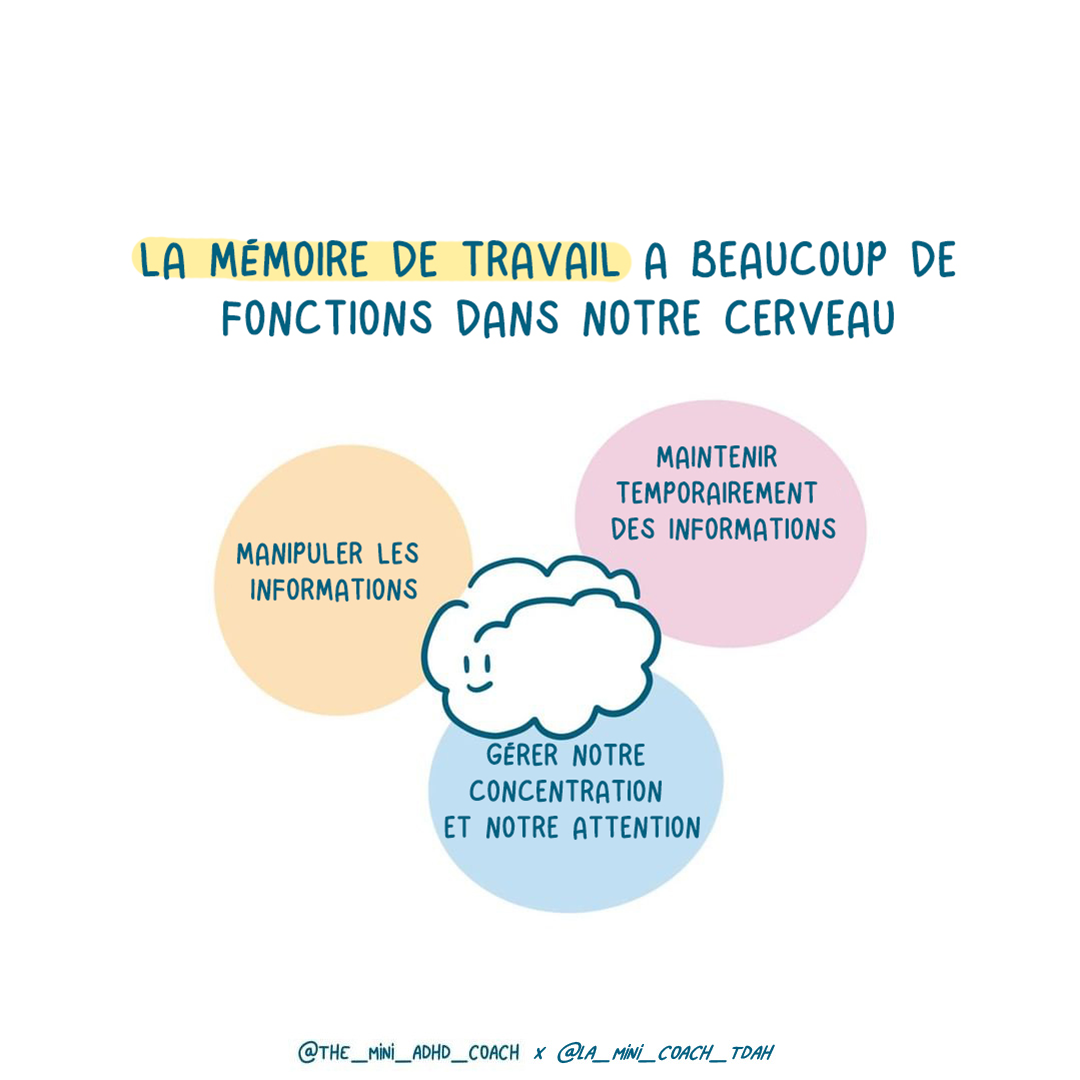
\includegraphics[width=0.7\textwidth]{images/ADHD-Working-Memory.png}
    \caption{Mémoire de Travail (TDAH)}
    \label{fig:tdah}
\end{figure}

\end{document}